\section{Theories of higher ranks}\label{sec:higher rank theories}

In this section, we apply our bootstrap approach for some interesting higher rank theories and compute their BPS spectra.


\subsection{\texorpdfstring{$SU(4)_8$}{SU(4)8}}\label{sec:SU(4)8}

The first example is the 5d $ SU(4) $ gauge theory with the CS level 8. This theory can be obtained from $\mathbb{Z}_3$ automorphism twist of the 6d minimal $SO(8)$ SCFT
\begin{align}
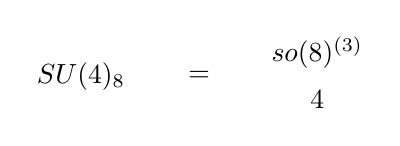
\begin{tikzpicture}
\draw (0, 0) node {$ SU(4)_8 $}
(1.5, 0) node {$ = $}
(3, 0.3) node {$ \mathfrak{so}(8)^{(3)} $}
(3, -0.3) node {$ 4 $}
;
\end{tikzpicture}
\end{align}
It has a geometric realization as \cite{Bhardwaj:2019fzv}
\begin{align}\label{eq:su4_8_geo}
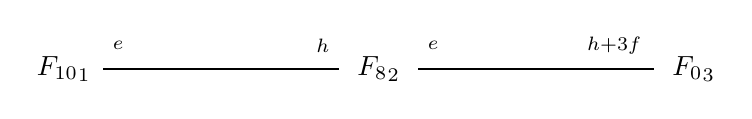
\begin{tikzpicture}
\draw (0, 0) node {$ \eval{\mathbb{F}_{10}}_1 $}
(4, 0) node {$ \eval{\mathbb{F}_8}_2 $}
(8, 0) node {$ \eval{\mathbb{F}_0}_3 $};
\draw [thick](0.5, 0) -- (3.5, 0);
\draw [thick] (4.5, 0) -- (7.5, 0);
\draw (0.7, 0.3) node {$ _{e} $}
(3.3, 0.3) node {$ _h $}
(4.7, 0.3) node {$ _e $}
(7, 0.3) node {$ _{h + 3f} $}
;
\end{tikzpicture}
\end{align}
It is convenient to use the volumes of primitive 2-cycles in the geometry \eqref{eq:su4_8_geo} as the basis in the computation below,
\begin{align}\label{eq:su4_8_vol}
&\vol (f_1) = 2\phi_1 - \phi_2, 
&&\vol (f_2) = -\phi_1 + 2\phi_2 - \phi_3, \nonumber \\
&\vol (f_3) = -\phi_2 + 2\phi_3,
&&\vol (e_3) = -3\phi_2 + 2\phi_3 + m_0.
\end{align}

We will now solve the blowup equations in both the 5d $SU(4)$ and 6d $SO(8)$ descriptions. In the 5d description, the effective prepotential on the $\Omega$-background is given by
\begin{align}\label{eq:su4_8_prepotential}
\mathcal{E} = & ~\frac{1}{\epsilon_1 \epsilon_2} \qty( \mathcal{F} - \frac{\epsilon_1^2 + \epsilon_2^2}{12} \qty(\phi_1 +\phi_2 +\phi_3) + \epsilon_+^2 (\phi_1 + \phi_2+ \phi_3) )\,, \nonumber \\
6\mathcal{F}
=&~ 8\phi_1^3 + 24\phi_1^2 \phi_2 - 30\phi_1 \phi_2^2 + 8\phi_2^3 + 18\phi_2^2 \phi_3 - 24\phi_2 \phi_3^2 + 8\phi_3^3 \nonumber \\
& + m_0 (\phi_1^2 - \phi_1 \phi_2 + \phi_2^2 - \phi_2 \phi_3 + \phi_3^2)\ ,
\end{align}
where $ m_0 $ is the $SU(4)$ gauge coupling. We find a set of consistent magnetic fluxes as
\begin{align}
n_i \in \mathbb{Z} \ , \quad
B_{m_0} = 0 \ ,
\end{align}
which provides a solvable unity blowup equation. The solution to the blowup equation is summarized in Table~\ref{table:SU4_8}.

We now turn to the 6d description. The subalgebra $G_2$ of $\mathfrak{so}(8)$ is invariant under the $\mathbb{Z}_3$ twist. So in the 5d reduction the 6d $SO(8)$ vector multiplet is decomposed into a $ G_2 $ adjoint with KK charge 0 and two $ G_2 $ fundamentals with KK charges $\tau/3,2\tau/3 $. The perturbative contribution to the GV-invariant is thus given by
\begin{align}
\mathcal{Z}_{\text{1-loop}}
= \PE \Bigg[-\frac{1+p_1 p_2}{(1-p_1)(1-p_2)} \frac{1}{1-q} &\bigg(\sum_{e \in \mathbf{R}^+} e^{-e\cdot \phi} + q^{1/3} \sum_{w \in \mathbf{F}} e^{-w\cdot \phi} \nonumber \\
& + q^{2/3} \sum_{w \in \mathbf{F}} e^{-w\cdot \phi} +  q\sum_{e\in \mathbf{R}^+} e^{e\cdot\phi}\bigg) \Bigg]\,,
\end{align}
where $ \mathbf{R}^+ $ denotes the positive roots and $ \mathbf{F} $ denotes the weights in the fundamental representation of $ G_2 $ algebra. See Appendix~\ref{appendix:1-loop} for more details.

The effective prepotential in the 6d description reads
\begin{align}
\mathcal{E} &= \frac{1}{\epsilon_1 \epsilon_2} \qty( \mathcal{F}_{\mathrm{tree}} + \mathcal{F}_{\text{1-loop}} - \frac{\epsilon_1^2 + \epsilon_2^2}{12}(\phi_1 + \phi_2) + \epsilon_+^2 (\phi_1 + \phi_2 ) )\ , \nonumber \\
\mathcal{F}_{\mathrm{tree}} &= 2\tau \phi_0^2 + \phi_0 \qty(12\phi_1^2 - 12\phi_1 \phi_2 + 4\phi_2^2 -\frac{\epsilon_1^2 + \epsilon_2^2}{2} + 6\epsilon_+^2)\ , \nonumber \\
\mathcal{F}_{\text{1-loop}} &= \frac{4}{3}\phi_1^3 + 3\phi_1^2 \phi_2 - 4\phi_1 \phi_2^2 + \frac{4}{3}\phi_2^3 - \frac{5}{9}\tau (3\phi_1^2 - 3\phi_1 \phi_2 + \phi_2^2) \ . \label{eq:1-loopSO8Aut}
\end{align}
One can check that after taking the shifts $ \phi_1 \to \phi_1 - 2\phi_0 $, $ \phi_2 \to \phi_2 - 3\phi_0 $, where the coefficients of $ \phi_0 $ are the dual Coxeter labels of affine $ D_4^{(3)} $ algebra, the cubic prepotential $\mathcal{F}_{\text{1-loop}}$ reproduces the triple intersection numbers of compact 4-cycles in the geometry \eqref{eq:su4_8_geo}. Also, the 5d effective prepotential in \eqref{eq:su4_8_prepotential} agrees with this 6d effective prepotential after redefining the 5d parameters as 
\begin{align}
\phi_1 \to \phi_0 + \frac{\tau}{9}, \quad
\phi_2 \to \phi_1 + 2\phi_0 - \frac{\tau}{9}, \quad
\phi_3 \to \phi_2 + 3\phi_0 - \frac{\tau}{3}, \quad
m_0 \to \frac{\tau}{3},
\end{align}
up to constant terms.

To compute the BPS spectrum (or the elliptic genus), we can use three unity blowup equations with three sets of consistent magnetic fluxes given by
\begin{align}
n_{1, 2} \in \mathbb{Z} \ , \quad
B_\tau = 0 \ , \quad
n_0 \in \mathbb{Z} + B_0 \quad (B_0 = -1/4,\ 0,\ 1/4) \ ,
\end{align}
which preserve the affine $ D_4^{(3)} $ structure. We can expand the three blowup equations in terms of the instanton string number and solve them at each order to find a closed expression for the elliptic genus of $k$-instanton strings, which is a similar procedure we did for the 6d $ SU(3) $ gauge theory with $ \mathbb{Z}_2 $ twist in section~\ref{subsubsec:SU3/Z2}.
\begin{table}
	\centering
	\begin{tabular}{|c|C{25ex}||c|C{25ex}|} \hline
		$\mathbf{d}$ & $\oplus N_{j_l, j_r}^{\mathbf{d}} (j_l, j_r)$ & $\mathbf{d}$ & $\oplus N_{j_l, j_r}^{\mathbf{d}} (j_l, j_r)$ \\ \hline
		$ (1, 0, 0, 0) $ & $ (0, \frac{1}{2}) $ & $ (1, 0, 0, 1) $ & $ (0, \frac{3}{2}) $ \\ \hline
		$ (1, 0, 0, 2) $ & $ (0, \frac{5}{2}) $ & $ (1, 0, 1, 0) $ & $ (0, \frac{1}{2}) $ \\ \hline
		$ (1, 0, 1, 1) $ & $ (0, \frac{1}{2}) \oplus (0, \frac{3}{2}) $ & $ (1, 0, 1, 2) $ & $ (0, \frac{3}{2}) \oplus (0, \frac{5}{2}) $ \\ \hline
		$ (1, 0, 2, 0) $ & $ (0, \frac{1}{2}) $ & $ (1, 0, 2, 1) $ & $ (0, \frac{1}{2}) \oplus (0, \frac{3}{2}) $ \\ \hline
		$ (1, 0, 2, 2) $ & $ (0, \frac{1}{2}) \oplus (0, \frac{3}{2}) \oplus (0, \frac{5}{2}) $ & $ (1, 1, 1, 0) $ & $ (0, \frac{1}{2}) $ \\ \hline
		$ (1, 1, 1, 1) $ & $ (0, \frac{1}{2}) \oplus (0, \frac{3}{2}) $ & $ (1, 1, 1, 2) $ & $ (0, \frac{3}{2}) \oplus (0, \frac{5}{2}) $ \\ \hline
		$ (1, 1, 2, 1) $ & $ 2(0, \frac{1}{2}) \oplus (0, \frac{3}{2}) $ & $ (1, 1, 2, 2) $ & $ (0, \frac{1}{2}) \oplus 2(0, \frac{3}{2}) \oplus (0, \frac{5}{2}) $ \\ \hline
		$ (1, 2, 2, 0) $ & $ (0, \frac{1}{2}) $ & $ (1, 2, 2, 1) $ & $ (0, \frac{1}{2}) \oplus (0, \frac{3}{2}) $ \\ \hline
		$ (1, 2, 2, 2) $ & $ (0, \frac{1}{2}) \oplus (0, \frac{3}{2}) \oplus (0, \frac{5}{2}) $ & $ (2, 0, 0, 1) $ & $ (0, \frac{5}{2}) $ \\ \hline
		$ (2, 0, 0, 2) $ & $ (0, \frac{5}{2}) \oplus (0, \frac{7}{2}) \oplus (\frac{1}{2}, 4) $ & $ (2, 0, 1, 1) $ & $ (0, \frac{3}{2}) \oplus (0, \frac{5}{2}) $ \\ \hline
		$ (2, 0, 1, 2) $ & $ (0,\frac{3}{2}) \oplus 3(0,\frac{5}{2}) \oplus 2(0,\frac{7}{2}) \oplus 1(\frac{1}{2},3) \oplus (\frac{1}{2},4) $ & $ (2, 0, 2, 1) $ & $ (0,\frac{1}{2}) \oplus (0,\frac{3}{2}) \oplus (0,\frac{5}{2}) $ \\ \hline
		$ (2, 0, 2, 2) $ & $ (0,\frac{1}{2}) \oplus 3(0,\frac{3}{2}) \oplus 4(0,\frac{5}{2}) \oplus 2(0,\frac{7}{2}) \oplus (\frac{1}{2},2) \oplus (\frac{1}{2},3) \oplus (\frac{1}{2},4) $ & $ (2, 1, 1, 1) $ & $ (0, \frac{3}{2}) \oplus (0, \frac{5}{2}) $ \\ \hline
		$ (2, 1, 2, 1) $ & $ (0, \frac{1}{2}) \oplus 2(0, \frac{3}{2}) \oplus (0, \frac{5}{2}) $ & $ (2, 1, 2, 2) $ & $ (0,\frac{1}{2}) \oplus 5(0,\frac{3}{2}) \oplus 7(0,\frac{5}{2}) \oplus 3(0,\frac{7}{2}) \oplus (\frac{1}{2},2) \oplus 2(\frac{1}{2},3) \oplus (\frac{1}{2},4) $ \\ \hline
		$ (2, 2, 2, 1) $ & $ (0, \frac{1}{2}) \oplus (0, \frac{3}{2}) \oplus (0, \frac{5}{2}) $ & $ (2, 2, 2, 2) $ & $ (0,\frac{1}{2}) \oplus 3(0,\frac{3}{2}) \oplus 4(0,\frac{5}{2}) \oplus 2(0,\frac{7}{2}) \oplus (\frac{1}{2},2) \oplus (\frac{1}{2},3) \oplus (\frac{1}{2},4) $ \\ \hline
	\end{tabular}
	\caption{BPS spectrum of the pure $ SU(4)_8 $ theory for $ d_i \leq 2 $. Here, $ \mathbf{d} = (d_1, d_2, d_3, d_4) $ labels the state with charge $ d_1 e_3 + d_2 f_1 + d_3 f_2 + d_4 f_3 $.} \label{table:SU4_8}
\end{table}
We checked in the K\"ahler parameter expansion that the 6d solution perfectly agrees with the 5d result in Table~\ref{table:SU4_8}.  


\subsection{\texorpdfstring{6d $ SO(8) $ gauge theory with $ \mathbb{Z}_2 $ twist}{6d SO(8) gauge theory with Z2 twist}}

We can also consider $ \mathbb{Z}_2 $ twisted compactification of the 6d minimal $ SO(8) $ SCFT. This theory has no 5d gauge theory description, but it has a geometric realization given by \cite{Bhardwaj:2019fzv}
\begin{align}
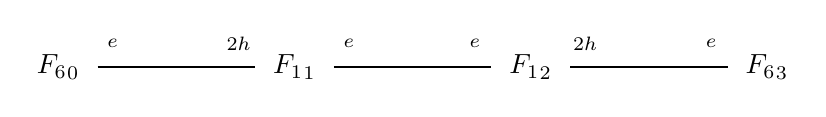
\begin{tikzpicture}\label{eq:so8/z2_geo}
\draw (0, 0) node {$ \eval{\mathbb{F}_{6}}_0 $}
(3, 0) node {$ \eval{\mathbb{F}_1}_1 $}
(6, 0) node {$ \eval{\mathbb{F}_1}_2 $}
(9, 0) node {$ \eval{\mathbb{F}_6}_3 $};
\draw [thick](0.5, 0) -- (2.5, 0)
(3.5, 0) -- (5.5, 0)
(6.5, 0) -- (8.5, 0);
\draw (0.7, 0.3) node {$ _{e} $}
(2.3, 0.3) node {$ _{2h} $}
(3.7, 0.3) node {$ _e $}
(5.3, 0.3) node {$ _e $}
(6.7, 0.3) node {$ _{2h} $}
(8.3, 0.3) node {$ _{e} $}
;
\end{tikzpicture}
\end{align}

Upon this compactification, the 6d $SO(8)$ gauge field is decomposed into a 5d gauge field in the adjoint representation and another 5d field carrying KK-charge $\frac{1}{2}$ in the fundamental representation of the invariant subalgebra $ \mathfrak{so}(7)$. The perturbative part of the GV-invariant in this theory can then be written as
\begin{align}
Z_{\mathrm{1-loop}}
= \PE \qty[-\frac{1+p_1 p_2}{(1-p_1)(1-p_2)} \frac{1}{1-q} \qty( \sum_{e \in \mathbf{R}^+} e^{-w\cdot \phi} + q^{1/2} \sum_{w \in \mathbf{F}} e^{-w\cdot \phi} + q \sum_{e \in \mathbf{R}^+} e^{w\cdot \phi} ) ] \ ,
\end{align}
where  $ \mathbf{R}^+ $ denotes the positive roots and $ \mathbf{F} $ denotes the fundamental weights of the $ \mathfrak{so}(7) $ algebra.

The effective prepotential on the $\Omega$-background reads
\begin{align}
\mathcal{E} &= \frac{1}{\epsilon_1 \epsilon_2} \qty( \mathcal{F}_{\mathrm{tree}} + \mathcal{F}_{\text{1-loop}} - \frac{\epsilon_1^2 + \epsilon_2^2}{12}(\phi_1 + \phi_2 + \phi_3) +\epsilon_+^2 (\phi_1 + \phi_2 + \phi_3)  ) \ , \nonumber \\
\mathcal{F}_{\mathrm{tree}} &= 2\tau \phi_0^2 + \phi_0 \qty(4\phi_1^2 - 4\phi_1 \phi_2 + 4\phi_2^2 - 8\phi_2 \phi_3 + 8\phi_3^2 -\frac{\epsilon_1^2 + \epsilon_2^2}{2} + 6\epsilon_+^2)\ , \nonumber \\
\mathcal{F}_{\text{1-loop}} &= \frac{4}{3}\phi_1^3 - \frac{1}{2} \phi_1^2 \phi_2 - \frac{1}{2} \phi_1 \phi_2^2 + \frac{4}{3}\phi_2^3 - 3\phi_2^2 \phi_3 + 2\phi_2 \phi_3^2 + \frac{4}{3}\phi_3^3 \nonumber \\
& \quad  - \frac{3}{4}\tau (\phi_1^2 - \phi_1 \phi_2 + \phi_2^2 - 2\phi_2 \phi_3 + 2\phi_3^2)\ .
\end{align}
One can easily check that the cubic prepotential reproduces the triple intersection numbers of compact 4-cycles in the geometry \eqref{eq:so8/z2_geo} by shifting $ \phi_1 \to \phi_1 - 2\phi_0 $, $ \phi_2 \to \phi_2 - 2\phi_0 $ and $ \phi_3 \to \phi_3 - \phi_0 $.

We find three unity blowup equations from the 3 sets of consistent magnetic fluxes:
\begin{align}
n_{1, 2, 3} \in \mathbb{Z}\ , \quad
B_\tau = 0 \ , \quad
n_0 \in \mathbb{Z} + B_0 \quad (B_0 = -1/8,\ 1/8,\ 3/8) \ .
\end{align}
One can solve these three blowup equations together at each string order and compute a closed expression of the elliptic genus of the 6d $ SO(8) $ gauge theory with $ \mathbb{Z}_2 $ twist. The solution is shown in Table~\ref{table:SO8/Z2}. We checked that this result agrees with the BPS spectrum computed using topological vertex as well as the ADHM calculations in \cite{Kim:2021cua}.
\begin{table}
	\centering
	\begin{tabular}{|c|C{23ex}||c|C{23ex}|} \hline
		$\mathbf{d}$ & $\oplus N_{j_l, j_r}^{\mathbf{d}} (j_l, j_r)$ & $\mathbf{d}$ & $\oplus N_{j_l, j_r}^{\mathbf{d}} (j_l, j_r)$ \\ \hline
		$ (1, 0, 2, 3, 3) $ & $ (0, 0) $ & $ (1, 0, 3, 3, 3) $ & $ (0, 1) $ \\ \hline
		$ (1, \frac{1}{2}, 2, 2, 2) $ & $ (0, 0) \oplus (0, 1) $ & $ (1, \frac{1}{2}, 2, 3, 2) $ & $ (0, 0) \oplus (0, 1) $ \\ \hline
		$ (1, \frac{1}{2}, 2, 3, 3) $ & $ (0, 0) \oplus (0, 1) $ & $ (1, \frac{1}{2}, 3, 2, 2) $ & $ (0, 1) \oplus (0, 2) $ \\ \hline
		$ (1, \frac{1}{2}, 3, 3, 2) $ & $ (0, 0) \oplus 2(0, 1) \oplus (0, 2) $ & $ (1, \frac{1}{2}, 3, 3, 3) $ & $ (0, 0) \oplus 2(0, 1) \oplus (0, 2) $ \\ \hline
		$ (1, 1, 1, 1, 1) $ & $ (0, 1) $ & $ (1, 1, 1, 2, 1) $ & $ (0, 0) \oplus (0, 1) $ \\ \hline
		$ (1, 1, 1, 2, 2) $ & $ (0, 0) \oplus (0, 1) $ & $ (1, 1, 1, 2, 3) $ & $ (0, 0) \oplus (0, 1) $ \\ \hline
		$ (1, 1, 1, 3, 1) $ & $ (0, 1) \oplus (0, 2) $ & $ (1, 1, 1, 3, 2) $ & $ (0, 0) \oplus 2(0, 1) \oplus (0, 2) $ \\ \hline
		$ (1, 1, 1, 3, 3) $ & $ 2(0, 0) \oplus 3(0, 1) \oplus (0, 2) $ & $ (1, 1, 2, 1, 1) $ & $ (0, 0) \oplus (0, 1) \oplus (0, 2) $ \\ \hline
		$ (1, 1, 2, 2, 1) $ & $ 2(0, 0) \oplus 3(0, 1) \oplus (0, 2) $ & $ (1, 1, 2, 2, 2) $ & $ 2(0, 0) \oplus 3(0, 1) \oplus (0, 2) $ \\ \hline
		$ (1, 1, 2, 2, 3) $ & $ 2(0, 0) \oplus 3(0, 1) \oplus (0, 2) $ & $ (1, 1, 2, 3, 1) $ & $ \! 2(0, 0) \oplus 3(0, 1) \oplus 2(0, 2) \! $ \\ \hline
		$ (1, 1, 2, 3, 2) $ & $ \! 4(0, 0) \oplus 6(0, 1) \oplus 2(0, 2) \! $ & $ (1, 1, 2, 3, 3) $ & $ 9(0, 0) \oplus 11(0, 1) \oplus 3(0, 2) \oplus (\frac{1}{2}, \frac{1}{2}) $ \\ \hline
		$ (1, 1, 3, 1, 1) $ & $ (0, 1) \oplus (0, 2) \oplus (0, 3) $ & $ (1, 1, 3, 2, 1) $ & $ (0, 0) \oplus 3(0, 1) \oplus 3(0, 2) \oplus (0, 3) $ \\ \hline
		$ (1, 1, 3, 2, 2) $ & $ (0, 0) \oplus 3(0, 1) \oplus 3(0, 2) \oplus (0, 3) $ & $ (1, 1, 3, 2, 3) $ & $ (0, 0) \oplus 3(0, 1) \oplus 3(0, 2) \oplus (0, 3) $ \\ \hline
		$ (1, 1, 3, 3, 1) $ & $ 2(0, 0) \oplus 5(0, 1) \oplus 3(0, 2) \oplus (0, 3) $ & $ (1, 1, 3, 3, 2) $ & $ 4(0, 0) \oplus 8(0, 1) \oplus 5(0, 2) \oplus (0, 3) $ \\ \hline
		$ (1, 1, 3, 3, 3) $ & \multicolumn{3}{c|}{$ 8(0, 0) \oplus 17(0, 1) \oplus 10(0, 2) \oplus 2(0, 3) \oplus (\frac{1}{2}, \frac{1}{2}) \oplus (\frac{1}{2}, \frac{3}{2}) $} \\ \hline
	\end{tabular}
	\caption{BPS spectrum of $ SO(8) $ gauge theory with $ \mathbb{Z}_2 $ twist for $ d_1 = 1 $, $ d_2 \leq 1 $ and $ d_{3,4, 5} \leq 3 $. Here, $ \mathbf{d} = (d_1, d_2, d_3, d_4, d_5) $ labels BPS states with charge $ d_1 \Phi + d_2 \tau + d_3 \alpha_1 + d_4 \alpha_2 + d_5 \alpha_3 $, where $ \alpha_1 = 2\phi_1-\phi_2 $, $ \alpha_2 = -\phi_1 + 2\phi_2 - 2\phi_3 $, $ \alpha_3 = -\phi_2 + 2\phi_3 $ are simple roots of $ \mathfrak{so}(7) $ algebra.} \label{table:SO8/Z2}
\end{table}


\subsection{\texorpdfstring{$ SU(5)_8 $: undetermined}{SU(5)8}}

Our last example is the 5d $ SU(5) $ gauge theory with the CS level $ 8 $. This theory was classified as an `undetermined theory' in \cite{Bhardwaj:2020gyu} since its UV completion has not been identified. Following our bootstrapping procedure, we found that this theory may have no consistent UV completion. We now explain it below.

To begin with, the geometric realization of this theory is given by 
\begin{align}\label{eq:su5_8}
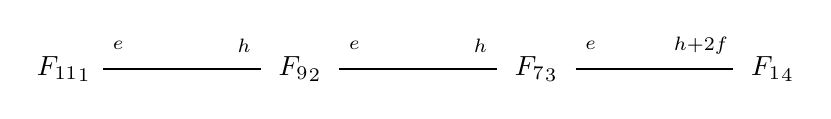
\begin{tikzpicture}
\draw (0, 0) node {$ \eval{\mathbb{F}_{11}}_1 $}
(3, 0) node {$ \eval{\mathbb{F}_9}_2 $}
(6, 0) node {$ \eval{\mathbb{F}_7}_3 $}
(9, 0) node {$ \eval{\mathbb{F}_1}_4 $};
\draw [thick](0.5, 0) -- (2.5, 0)
(3.5, 0) -- (5.5, 0)
(6.5, 0) -- (8.5, 0);
\draw (0.7, 0.3) node {$ _{e} $}
(2.3, 0.3) node {$ _{h} $}
(3.7, 0.3) node {$ _e $}
(5.3, 0.3) node {$ _h $}
(6.7, 0.3) node {$ _{e} $}
(8.1, 0.3) node {$ _{h+2f} $}
;
\end{tikzpicture} \, .
\end{align}
However, this geometry is not shrinkable because it does not have  non-trivial Coulomb branch where the volumes of primitive 2-cycles 
\begin{align}\label{eq:su5_8_vol}
\vol (f_1) & = 2\phi_1 - \phi_2, \quad
&\vol (f_2) &= -\phi_1 + 2\phi_2 - \phi_3, \quad
&\vol (f_3) &= -\phi_2 + 2\phi_3 - \phi_4, \nonumber \\
\vol (f_4) &= -\phi_3 + 2\phi_4, \quad
&\vol (e_4) &= -2\phi_3 + \phi_4 + m_0,&&
\end{align}
are all non-negative simultaneously in the UV limit where $ m_0 \to 0 $. Thus, from the geometric perspective, it is unclear whether this theory is UV completable or not.

\begin{table}
	\centering
	\begin{tabular}{|c|C{25ex}||c|C{25ex}|} \hline
		$\mathbf{d}$ & $\oplus N_{j_l, j_r}^{\mathbf{d}} (j_l, j_r)$ & $\mathbf{d}$ & $\oplus N_{j_l, j_r}^{\mathbf{d}} (j_l, j_r)$ \\ \hline
			$ (1, 0, 0, 0, 0) $ & $ (0, 0) $ & $ (1, 0, 0, 0, 1) $ & $ (0, 1) $ \\ \hline
			$ (1, 0, 0, 0, 2) $ & $ (0, 2) $ & $ (1, 0, 0, 1, 0) $ & $ (0, 0) $ \\ \hline
			$ (1, 0, 0, 1, 1) $ & $ (0, 0) \oplus (0, 1) $ & $ (1, 0, 0, 1, 2) $ & $ (0, 1) \oplus (0, 2) $ \\ \hline
			$ (1, 0, 1, 1, 0) $ & $ (0, 0) $ & $ (1, 0, 1, 1, 1) $ & $ (0, 0) \oplus (0, 1) $  \\ \hline
			$ (1, 0, 1, 1, 2) $ & $ (0, 1) \oplus (0, 2) $ & $ (1, 1, 1, 1, 0) $ & $ (0, 0) $ \\ \hline
			$ (1, 1, 1, 1, 1) $ & $ (0, 0) \oplus (0, 1) $ & $ (2, 0, 0, 0, 2) $ & $ (0, \frac{5}{2}) $ \\ \hline
			$ (2, 0, 0, 1, 2) $ & $ (0, \frac{3}{2}) \oplus (0, \frac{5}{2}) $ & $ (2, 0, 1, 1, 2) $ & $ (0, \frac{3}{2}) \oplus (0, \frac{5}{2}) $ \\ \hline
			$ (2, 1, 1, 1, 2) $ & $ (0, \frac{3}{2}) \oplus (0, \frac{5}{2}) $ & $ \vdots$ & $ \vdots $ \\ \hline
			$ \vdots $ & $ \vdots $ & $ (6, 1, 4, 8, 2) $ & $ (0, \frac{1}{2}) $ \\ \hline
	\end{tabular}
	\caption{BPS spectrum of the pure $ SU(5)_8 $ theory up to $ d_1, d_5 \leq 2 $, $ d_2, d_3, d_4 \leq 1$ together with the negative volume state of $ \mathbf{d} = (6, 1, 4, 8, 2) $. Here, $ \mathbf{d} = (d_1, d_2, d_3, d_4, d_5) $ labels state with charge $ d_1 e_4 + d_2 f_1 + d_3 f_2 + d_4 f_3 + d_5 f_4 $.} \label{table:SU5_8}
\end{table}

Let us try to solve blowup equations and compute the BPS spectrum of this theory. The effective prepotential for the theory is given by
\begin{align}
\mathcal{E} 
&= \frac{1}{\epsilon_1 \epsilon_2} \qty( \mathcal{F} -\frac{\epsilon_1^2 + \epsilon_2^2}{12}(\phi_1 + \phi_2 + \phi_3 + \phi_4) + \epsilon_+^2 (\phi_1 + \phi_2 + \phi_3 + \phi_4)) \, ,
\nonumber \\
6\mathcal{F}
&= 8\phi_1^3 + 27\phi_1^2 \phi_2 - 33\phi_1 \phi_2^2 + 8\phi_2^3 + 21\phi_2^2 \phi_3 - 27\phi_2 \phi_3^2 + 8\phi_3^3 + 15\phi_3^2 \phi_4 \nonumber \\
& \quad - 21\phi_3 \phi_4^2 + 8\phi_4^3 + 6m_0 (\phi_1^2 - \phi_1 \phi_2 + \phi_2^2 - \phi_2 \phi_3 + \phi_3^2 - \phi_3 \phi_4 + \phi_4^2) \, .
\end{align}
We can set a (trial) unity blowup equation using the following set of magnetic fluxes:
\begin{align}
n_i \in \mathbb{Z} \, , \quad
B_{m_0} = 1/2 \, .
\end{align}
The solution to the blowup equation is summarized in Table \ref{table:SU5_8}.
The solution  involves many negative volume hypermultiplet states at one- and three-instanton orders. As explained, we should flop such states to move on to a unitary chamber where all the BPS states have non-negative masses. For instance, the instantonic hypermultiplets with charges $e_4$, $e_4+f_3$, and $e_4+f_2+f_3$ in Table \ref{table:SU5_8} should be flopped.

After a series of flop transitions, we find that all the BPS states up to certain higher orders can be written as non-negative linear combinations of basis curves given by
\begin{align}\label{eq:SU58floppedNewBasis}
\{ &-e_4 - 2f_1 - 2f_2 - 2f_3,\ -3e_4 - 2f_2 - 4f_3 - f_4,\  -3e_4 - f_1 - f_2 - 4f_3 -f_4, \nonumber \\
&3e_4 + 2f_2 + 5f_3 + f_4,\   6e_4 + f_1 + 4f_2 + 8f_3 + 2f_4  \} \, .
\end{align}
Here the minus signs in the first three curves indicate that the associated hypermultiplets, which exist in the spectrum, are flopped. The spectrum also involves a BPS hypermultiplet wrapping the fourth curve $ 3e_4 + 2f_1 + 5f_3 + f_4 $.

The higher order solution shows that there exists a vector multiplet wrapping the last curve $ 6e_4 + f_1 + 4f_2 + 8f_3 + 2f_4 $. One can then check that the volume of this curve cannot be non-negative while satisfying the non-negative volume conditions $ \vol(f_i) \geq 0 $ for the perturbative vector multiplets. Unfortunately we cannot flop vector multiplets. This implies that the theory with the spectrum we obtained from the blowup equation has no unitary chamber where masses of all the BPS states are non-negative. One may wonder if the $SU(5)_8$ theory has other choices of magnetic fluxes leading to physically consistent BPS spectrum, but we could not find any other solvable blowup equation for this theory. Thus our computation suggests that the 5d $ SU(5)_8 $ theory may have no UV completion.